\documentclass[paper=a4, fontsize=11pt]{scrartcl}
\renewcommand{\baselinestretch}{1.5} 


\usepackage[english]{babel}															% English language/hyphenation
\usepackage[protrusion=true,expansion=true]{microtype}	
\usepackage{amsmath,amsfonts,amsthm} % Math packages
\usepackage[pdftex]{graphicx}	
\usepackage{pdfpages}

\usepackage{tabularx}




%%% Custom sectioning
%\allsectionsfont{\centering \normalfont\scshape}


%%% Custom headers/footers (fancyhdr package)
\usepackage{fancyhdr}
\pagestyle{fancyplain}
\fancyhead{}											% No page header
\fancyfoot[L]{}											% Empty 
\fancyfoot[C]{}											% Empty
\fancyfoot[R]{\thepage}									% Pagenumbering
\renewcommand{\headrulewidth}{0pt}			% Remove header underlines
\renewcommand{\footrulewidth}{0pt}				% Remove footer underlines
\setlength{\headheight}{13.6pt}


%%% Equation and float numbering
\numberwithin{equation}{section}		% Equationnumbering: section.eq#
\numberwithin{figure}{section}			% Figurenumbering: section.fig#
\numberwithin{table}{section}				% Tablenumbering: section.tab#


% % %subsubsub
%\documentclass{article}
\makeatletter
\renewcommand\paragraph{\@startsection{paragraph}{4}{\z@}%
            {-2.5ex\@plus -1ex \@minus -.25ex}%
            {1.25ex \@plus .25ex}%
            {\normalfont\normalsize\bfseries}}
\makeatother
\setcounter{secnumdepth}{4} % how many sectioning levels to assign numbers to
\setcounter{tocdepth}{4}    % how many sectioning levels to show in ToC

% %end subsubsub

\renewcommand{\labelitemi}{$\star$}


%%% Maketitle metadata
\newcommand{\horrule}[1]{\rule{\linewidth}{#1}} 	% Horizontal rule

\title{
		%\vspace{-1in} 	
		\usefont{OT1}{bch}{b}{n}
		\normalfont \normalsize \textsc{SOFTWARE ENGINEERING 2018} \\ [25pt]
		\horrule{1.2pt} \\[0.4cm]
		
\includegraphics[width = \textwidth]{Logo.png} \\\huge Student Mark Management Portal \\
		\horrule{2pt} \\[0.5cm]
}
\author{
		\normalfont 					
       \normalsize Zakiya Safi 1319070\\
       \normalsize Ahmed Ali Karani 1036074 \\
       \normalsize Zubair Ahmed Bulbulia 1249593 \\
        \normalsize Kyle Morris 1112649\\\\[-3pt]	}	\normalsize      
 \date{5 October 2018}



%%% Begin document
\begin{document}

\maketitle
\newpage

\tableofcontents

\newpage

\section{Introduction}
The following report document contains the software information of a Student mark management system, affectionately named Gr(A+)der. Within this report, all necessary system design is covered, namely: project model, all system framework information, project scope and use cases. Furthermore, the system implementation includes testing, task-responsibility breakdown, as well as all functional system layers. 

\subsection{Project Definition}
It is required to develop and implement a student mark system, which allows a convenient, user-friendly way for staff to record marks, and students to view marks.

\subsection{Problem Statement}
We require all available marks corresponding to a specific student number to be visible by that student.\\
Student marks must only be viewable by users who have access to them.\\
Marks must only be able to be uploaded, and edited by administrative personnel.\\\\
Thus, one of the most important tasks is the restriction of access to certain users. We will thus implement access control in the form of username/password combinations that achieve the above during the login process.


\subsection{Project Objective}
The portal needs to produce an efficient, user-friendly system which ensures the following:

\begin{itemize}
\item A student can view their available marks
\item A student can query their marks
\item A student can only view their own marks \\
\item Administrative personnel can upload and modify marks.
\end{itemize}

\subsection{Project Stakeholders}
Below is a list of stakeholders:

\begin{itemize}
\item Student
\item Course Coordinator
\item School Administrator
\item Database Administrator
\item System Administrator
\end{itemize}


% % % % % % % % % % % % %
% % % % % % % % % % % % % %

\section{Requirement Specifications}

\subsection{Project Scope}
The task requirement is to develop a web-based system with the capabilities of being able to
record marks of various assessments, for a multitude of students. It will thus function as a
database for all student marks, across various courses. On the front-end, it is required to
implement separate functionality and limitations for three different categories of user -
student, course coordinator and school administrator. There must exist the capability for
Course Coordinator and School Administrator to be able to access, edit and update marks
on the database, as well as being able to view student marks. From the student side, they
need to be able to view their marks from the 'portal'. They must also have the ability to query
a certain assignment mark if they believe there to be an error with it. Students must have the
limitation of not having access to other students' marks, and not being able to make
modifications to their own marks.
There are two back-end roles that need to be fulfilled: The database administrator, who is
responsible for ensuring the correct format of marks is recorded, that there are no erroneous
values stored, and that backups exist and are frequently maintained, and the Systems
administrator who is tasked with ensuring the correct system configuration is established, as
well as the security perspectives of the portal.

\subsection{Product Description}
The project requirement that the group is required to fulfil is that of the  Student Mark
Management System. ​ The end result will be a fully-functioning web portal where students
are able to view their marks for a number of courses.





\subsubsection{User Characteristics}
Below describes each user of the system, and how they interact with the system:\\\\\textbf{Student:}
The system will create and display all available marks for a student, in a user-friendly way. The system will allow the student to query marks as well as provide the student with marks that are required in future assessments to obtain a pass in the course.\\\\\textbf{Course Coordinator:}
The Course Coordinator will be able to add courses to the system, assessments pertaining to courses, and weightings of assessments. The Course Coordinator will also enrol students in courses and enter their marks per assessment. These functionalities will be provided by the system.\\\\\textbf{School Administrator:}
The system will provide the School Administrator with the same functionality as that of the Course Coordinator as well as additional functionality. The additional functionality includes generating statistics regarding the performance of courses the School Administrator is involved in as well as viewing information on plagiarism offences.



% % % % % % % % % % % % % %
\subsection{Formal Requirements Definition}
The group has been tasked with specifically creating a web-based application (herein
referred to as the portal). The portal will need to incorporate a fully functioning front-end
(User interface), which is simple for all users to navigate (user friendly), aesthetically
pleasing, produces the correct output, displays correctly formatted information on the student
portal page, and have the correctly implemented security features to grant and restrict
access to certain features and/or information, for particular users.
For the back-end (database) requirements, it is necessary to ensure the correct relationships
exist between the various tables. It is imperative to select the correct identifying keys
(primary and foreign), to ensure the correct relational organisation of database entries is
upheld and maintained. Correct data types for the different attribute values must be selected
(eg. to store marks/scores for assessments as numerical values rather than text values, to
allow the creation of mathematical results, summaries and interpretive statistics). The
database needs to be continuously maintained, backed-up and updated to ensure the best
user experience on the portal and to rectify any bugs or glitches that may have resulted from
incorrect data collection, storing or manipulation.

\subsubsection{Requirements}

The below tables will list and describe the requirements as understood by our Gr(A+)der system. Each table will list the requirements, divided into relevant categories, followed by columns that classify the requirement as either:\\
\textbf{F}: Functional (core functionality that is integral to the system) or,\\\textbf{NF}: Non-functional (the methods in which the core functionality will be delivered).\\\\ The further classification is then split up into:\\
\textbf{M}: Mandatory (requirements key to project success), or\\\textbf{O}: Optional (requirements that are not necessarily key to a successful project but may improve the final product).\\\\

%performance table
\begin{tabular}{|p{1cm}|p{9.5cm}|p{0.5cm}|p{0.5cm}|p{0.5cm}|p{0.5cm}|}
\hline  & \textbf{Performance Levels} & F & NF & M & O \\ 
\hline 1. & The system must handle all traffic levels without severely impacting the user experience. &  & X &  & X \\ 
\hline 2. & The system must work efficiently on all devices.  & X &  & X &  \\ 
\hline 3. &The system must be able to manage, and adapt to a growing database size, without causing major system disruption. &  & X &  & X \\ 
\hline 
\end{tabular} 
\\\\

%interface
\begin{tabular}{|p{1cm}|p{9.5cm}|p{0.5cm}|p{0.5cm}|p{0.5cm}|p{0.5cm}|}
\hline  & \textbf{Interface} & F & NF & M & O \\ 
\hline 1. & Provide an interface which allows users to access core    system functionality. & X &  & X &  \\ 
\hline 2. & Create a user-friendly interface that is intuitive for all system users.  &  & X &  & X \\
\hline 
\end{tabular} 
\\\\

%functional table
\begin{tabular}{|p{1cm}|p{9.5cm}|p{0.5cm}|p{0.5cm}|p{0.5cm}|p{0.5cm}|}
\hline  & \textbf{Functional Components} & F & NF & M & O \\ 
\hline 1. & Allow the Course Coordinator to add a course. & X &  & X &  \\ 
\hline 2. & Allow the Course Coordinator to enrol students.  & X &  & X &  \\ 
\hline 3. & Allow the Course Coordinator to add assessments. & X &  & X &  \\ 
\hline 4. & Allow the Course Coordinator to add or change a student mark in an assessment.  & X &  & X &  \\ 
\hline 5. & Generate statistics for the School Administrator. & X &  & X &  \\ 
\hline 6. & Allow the School Administrator to view offences. & X &  & X &  \\ 
\hline 7. & Provide students with results pertaining to assessments. & X &  & X &  \\ 
\hline 8. & Provide students with percentages required (in future assessments) to pass a course. & X &  & X &  \\ 
\hline 
\end{tabular} 
\\\\

%reliability
\begin{tabular}{|p{1cm}|p{9.5cm}|p{0.5cm}|p{0.5cm}|p{0.5cm}|p{0.5cm}|}
\hline  & \textbf{Reliability} & F & NF & M & O \\ 
\hline 1. & The system must always be available for students to view their marks. &  & X & X &  \\ 
\hline 2. & The system must provide all available marks to the student.  & X &  & X &  \\ 
\hline 3. & The system must consistently deliver accurate output to the user.  &  & X & X &  \\ 
\hline 
\end{tabular} 
\\\\

%security
\begin{tabular}{|p{1cm}|p{9.5cm}|p{0.5cm}|p{0.5cm}|p{0.5cm}|p{0.5cm}|}
\hline  & \textbf{Security} & F & NF & M & O \\ 
\hline 1. & A student should only be able to view his/her marks. &  & X & X &  \\ 
\hline 2. & An authentication system (involving a username and password) should be implemented in order to securely access personal information and ensure that lower level users cannot access higher level functionality.   &  & X & X &  \\ 
\hline 3. &The Course Coordinator should be restricted from School Administrator specific priorities.  &  & X & X &  \\ 
\hline 4. & The Student should be restricted from tasks that are specific to the Course Coordinator and School Administrator. & & X & X & \\
\hline 
\end{tabular} 
\\\\

%quality
\begin{tabular}{|p{1cm}|p{9.5cm}|p{0.5cm}|p{0.5cm}|p{0.5cm}|p{0.5cm}|}
\hline  & \textbf{Quality} & F & NF & M & O \\ 
\hline 1. & Provide a well polished system overall. &  & X & X &  \\ 
\hline 2. &  Provide a system with minimal bugs ensuring tasks are carried out correctly and consistently.  &  & X & X &  \\
\hline 
\end{tabular} 
\\


\subsubsection{Assumptions}
Below are defined the assumptions for each user type. In constructing the system, we assume the following: 

\paragraph{Student:}
\begin{itemize}
\item Student marks will be available from the portal.
\item Students feel comfortable logging into and using the web portal.
\item Students have an understanding of a web-based application and so understand
possible system delays.
\item Students make effective use of the system.
\end{itemize}

\paragraph{Course Coordinator:}
\begin{itemize}
\item CC will be responsible for uploading marks onto the database.
\item CC is comfortable with dealing with and making changes to the system.
\item CC understands how to apply a certain weighting to a course.
\end{itemize}

\paragraph{School Administrator:}
\begin{itemize}
\item SA knows how to navigate between different courses.
\item SA is comfortable with creating comparative statistics on different courses.
\item SA is able to identify students with offenses and can remove them from the course
(unenrol).
\end{itemize}

\paragraph{Database Administrator:}
\begin{itemize}
\item The database is correctly created with the appropriate relationships between entities
being implemented.
\item The data types of respective fields are appropriately defined.
\item Any erroneous data that appears during testing will be rectified.
\item Backups will be done regularly, and stored appropriately.
\end{itemize}

\paragraph{Systems Administrator:}
\begin{itemize}
\item The security of the system will ensure no ungranted access is provided to respective
users.
\item The system will communicate between the front and back-end without error. \\
\end{itemize}


\subsubsection{Dependencies}

The below describes vital information and system capabilities which are necessary for the system to run optimally:

\begin{itemize}
\item \textbf{Access to information:} In order for the system to fully function, we require access to certain university property. This is required as part of the initial system implementation, and is in the form of student, course, and assessment information.
\item \textbf{System resources:} We require the front and back ends of the system to effectively interact and communicate, in order for the system to correctly function.
 
\item \textbf{Internet connectivity:} It is required to have an internet connection in order for the system to request and access information off the remote server, and also for students to view their marks on the portal page.

\item \textbf{Database:}For the system to be operational it is necessary to have an integrated database with the correct student, course, and assessment information.

\item \textbf{Maths/Stats/Graphs:}Access to the Desmos/Plotly API or R for use for reporting purposes, to create graphs of course averages, etc.
\end{itemize}





\subsubsection{Operating Environment}

\paragraph{Operating System}
Any operating system that has the ability to view web-pages will work. This is due to the fact we are developing a web application. Thus, suitable OS’s include: Linux, Windows, iOS, Android, etc.

\paragraph{Architecture}
Web-based application; client-server web app.
Having a client-server architecture provides many useful advantages; namely having a centralised database management system located server-side provides an added layer of data access control and data security. It also allows for concurrent access and centralised processing. 

\paragraph{Database} 
\Huge\textbf{ADD HERE!!!!!!!}
\normalsize
\paragraph{Database Type}
Centralised (Database records will be on a main server).

\paragraph{Platform}
MVC. asp.net, x,y,. textbf{Theirs: “Python/Javascript/HTML/CSS”.} These components are used to create the web app which is accessible using an internet connection and a web browser.


\subsubsection{Data Management}
This concerns the storage of the input and output within the system. All data being used in the system will be stored in a database on a server provided by the University. The data will then be accessed by the logical layer and displayed through the interface layer of the 'Gr(A+)der' system. At this point the data will be informative.

\subsubsection{Portability}
The system should have the capabilities to run on any device that has a web browsing application without the need for additional browser plugins.       

% % % % % % % % %
\subsection{Use Cases}

\subsubsection{Use Case Set}
Below is a list of project Use Cases that were identified as being necessary for the system. They are organised according to the feature they relate do. The Use Cases have been structured in such a way to allow for more efficient administrative design to be implemented.

\paragraph{Core Use Cases}
These use cases represent the core functionality of our system.\\

\begin{tabular}{|l|l|}
\hline \textbf{Use Case} & \textbf{Actor}  \\ 
\hline View Marks  & Student  \\ 
\hline Query Marks & Student \\ 
\hline Upload Marks & Course Coordinator/ School Administrator \\ 
\hline Add Course & Course Coordinator/ School Administrator \\ 
\hline Add Assessment & Course Coordinator/ School Administrator \\ 
\hline Enrol Student & Course Coordinator/ School Administrator \\ 
\hline View Offenses & School Administrator \\ 
\hline 
\end{tabular} 

\paragraph{Reporting Use Cases}
These use cases are related to the integrated reporting capabilities of our system.\\

\begin{tabular}{|l|l|}
\hline \textbf{Use Case} & \textbf{Actor} \\
\hline View Comparative Reports & School Administrator \\
\hline View Course Reports & Course Coordinator \\
\hline
\end{tabular}\\

\paragraph{Maintenance Use Cases}
These use cases deal with the creation, deletion, viewing and updating of all other entities not included in the core use cases, but still required for the functionality of the system.\\

\begin{tabular}{|l|l|}
\hline \textbf{Use Case} & \textbf{Actor} \\
\hline Maintain Student & Course Coordinator/ School Administrator \\
\hline Maintain Course Coordinator & Course Coordinator/ School Administrator \\
\hline Maintain School Administrator & School Administrator \\
\hline
\end{tabular}


\subsubsection{Use Case Description}

\paragraph{Core Use Cases}

\textbf{View Marks}\\A student will select the “View Marks” option on their home page, accessible only after they have logged in. On doing so they will be presented with a list of all the courses for which they are enrolled. They will select a particular course, and will be able to see all the assessments for that particular course, and their marks for those assessments. They will also be able to view the mark(s) that need to be achieved on their remaining assessment(s) to achieve a pass for that particular course. \\\\ \textbf{Query Mark}\\While a student is viewing their marks, if they believe that their mark for an assessment is incorrect for any reason, they will select the “Query Mark” button associated with that particular assessment. They will then be asked to fill in a form explaining their reason for querying the mark. This query will then be sent to the respective Course Coordinator. A student is only allowed 3 ‘legitimate’ queries per year, and the system will ascribe an offense to a student if they submit a query which turns out to have no error. I.e if a student has ‘3 queries remaining’, they query a mark which has no error, they then lose a query (i.e. they then have 2), but if they query a mark which is an error, they keep that query. \\\\ \textbf{Upload Marks}\\A CC or SA will select the “Upload Marks” option on their home page, accessible only after they have logged in. They will then select a particular course and a particular assessment in that course. On doing so they will be presented with a list of all students enrolled in that course, and will then enter a mark for every student. When they click the “Save” button, these changes will be saved to the database.\\\\ \textbf{Add Course}\\A CC or SA will select the “Add Course” option on their respective homepages. They will then be presented with a form where they will have to fill in the details of the course, including the course name, course code, school, and course coordinator. If the CC is adding a course, they will automatically be set as the Course Coordinator. If the SA is adding a course they must select a course coordinator from a list of all the CCs on the system. Upon completing this form they will select the “Save” button and the new course and its details will be saved to the database.\\\\ \textbf{Add Assessment}\\From the homepage of the CC or SA, they will select to view courses. They will then be presented with a list of all their courses. When they select a particular course, they will be able to view all the assessments for that particular course, and add new assessments. When they select to add an assessment, they will be presented with a form where they must fill in the details for that particular assessment, including the assessment name, date, time, venue, total mark as well as the course percentage (the total percentage that this assessment contributes to the entire course). Upon completing this form they will select the “Save” button and the new course and its details will be saved to the database.\\\\ \textbf{Enrol Student}\\From the homepage of the CC or SA, they will select to view courses. They will then be presented with a list of all their courses. When they select a particular course, they will be able to view all the students enrolled in that particular course, and enrol new students in that course. When they select to enrol a student they will be presented with a form where they may enter the student IDs of the students to be enrolled. The system will cater for the user to enter a list of student IDs of many students who need to be enrolled, for the ease of the user. Once they select “Save”, these students will then be enrolled in the course and the changes will be saved to the database.\\\\ \textbf{View Offences}\\A SA will select the “View Offences” option on their homepage. They will then be presented with a list of all students who have committed an offence, as well as the details of the student offence, including the course, date and assessment.\\

\paragraph{Reporting Use Cases}
\textbf{View Course Reports}\\A CC  will select the “View Course Reports” option on their homepage. On doing so they will be presented with a list of all their courses. When they select a particular course, the report for that particular course will be displayed. \\\\ \textbf{View Comparative Reports}\\A SA will select the “View Course Reports” option on their homepage. On doing so they will be presented with a list of reports. When they select a particular report, that report will be displayed.

\paragraph{Maintenance Use Cases}
\textbf{Maintain Student}\\Includes the use cases Add Student, View Student, Update Student and Delete Student.\\\\ \textbf{Maintain Course Coordinator}\\Includes the use cases Add Course Coordinator, View Course Coordinator, Update Course Coordinator and Delete Course Coordinator.\\\\ \textbf{Maintain School Administrator}\\Includes the use cases Add School Administrator, View School Administrator, Update School Administrator and Delete School Administrator.\\\\ \textbf{Maintain Assessment}\\ Includes the use cases View Assessment, Update Assessment and Delete Assessment. (Not Add Assessment as this is already included and detailed in the core use case set).


% % % % % % % % % %
% % % % % % % % % % %

\section{System Design}

\subsection{Domain Model}

\subsubsection{Informal Description}
It is required to design and create a web-based system, which serves the primary purpose of allowing students to view university course marks. The system must be easy to use and navigate.\\\ The following functionality must exist:

\begin{itemize}
\item Students can login, view their uploaded marks, and query a mark.
\item Course coordinator can add/remove students to/from courses, upload marks, modify marks and allocate plagiarism and other offenses against a student.
\item School administrator can perform the same tasks as course coordinator (from an access point of view). Their main roles however concern comparative course mark results, and student offenses.
\end{itemize}



% % % % % % % % %
\subsection{System Use Cases}
Throughout the system, various scenarios are present, and exist. System use cases represent these scenarios.
\subsubsection{Final Use Case}
Following on from the initial Software Requirement Specification (SRS V2.1), the final project Use Case Set is defined below. Each case is separated by business feature, and further subdivided into feature.\\\\ \textbf{Core Use Cases:}
\begin{enumerate}
\item View Marks
\item Query Marks
\item Upload Marks
\item Add Course
\item Add Assessment
\item Enrol Student
\item View Offenses
\end{enumerate}
\textbf{Reporting Use Cases}
\begin{enumerate}
\item View Comparative Reports
\item View Course Reports
\end{enumerate}
\textbf{Maintenance Use Cases}
\begin{enumerate}
\item Maintain Student
\item Maintain Course Coordinator
\item Maintain School Administrator
\end{enumerate}

The list of Actors which will ink to the Use Case Set are as follows:
\begin{itemize}
\item Student
\item Course administrator
\item School administrator
\end{itemize}

\subsubsection{Use Case Diagram}
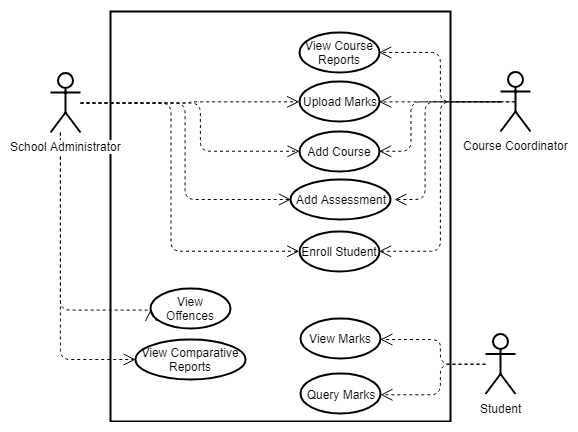
\includegraphics[width = \textwidth]{Use Case.png}\\\\ \textbf{Use case diagram explanation:}
Our system is comprised of 3 primary actors, as all actors are able to (in one way or another) make changes or directly interact with the system.\\The primary actors are student, course coordinator, and course administrator.\\The student can invoke the view marks and query mark use case, respectively.  This allows them to view the marks for all courses associated with their student number.\\ The course coordinator can invoke the View course report, Upload marks, Add course, Add assessment, and Enrol student use cases. This covers all administrative tasks involved with  mark recording and student enrolment.\\ School administrator is able to invoke the same use cases as the course coordinator, as well as being able to invoke View offenses, and View comparative report use case. Their primary role is concerned with student offenses, however, due to administrative privileges they are able to invoke same use cases as course coordinator.



\subsection{System Framework}
For the purpose of simplicity, the framework was divided into 3 key components, namely: Presentation, Business Logic and Data layer.

\subsubsection{System Architecture Overview}
Based on the requirement specification, group composition, time frame, and SCRUM Agile methodology chosen, the team has chosen the ASP.net Model View Controller (MVC) framework as the system architecture. \\\\MVC allows for:
\begin{itemize}
\item Separation of a system into three smaller components being the Data Layer (model), Presentation Layer (UI or view), and Business Logic Layer (controller).
\item Decoupling of modules enabling parallel development and separation of concerns.
\item Simpler integration in terms of implementation and deployment.
\item Usage of different languages (HTML,CSS,JavaScript,C\#).
\item Test Driven Development.
\end{itemize}

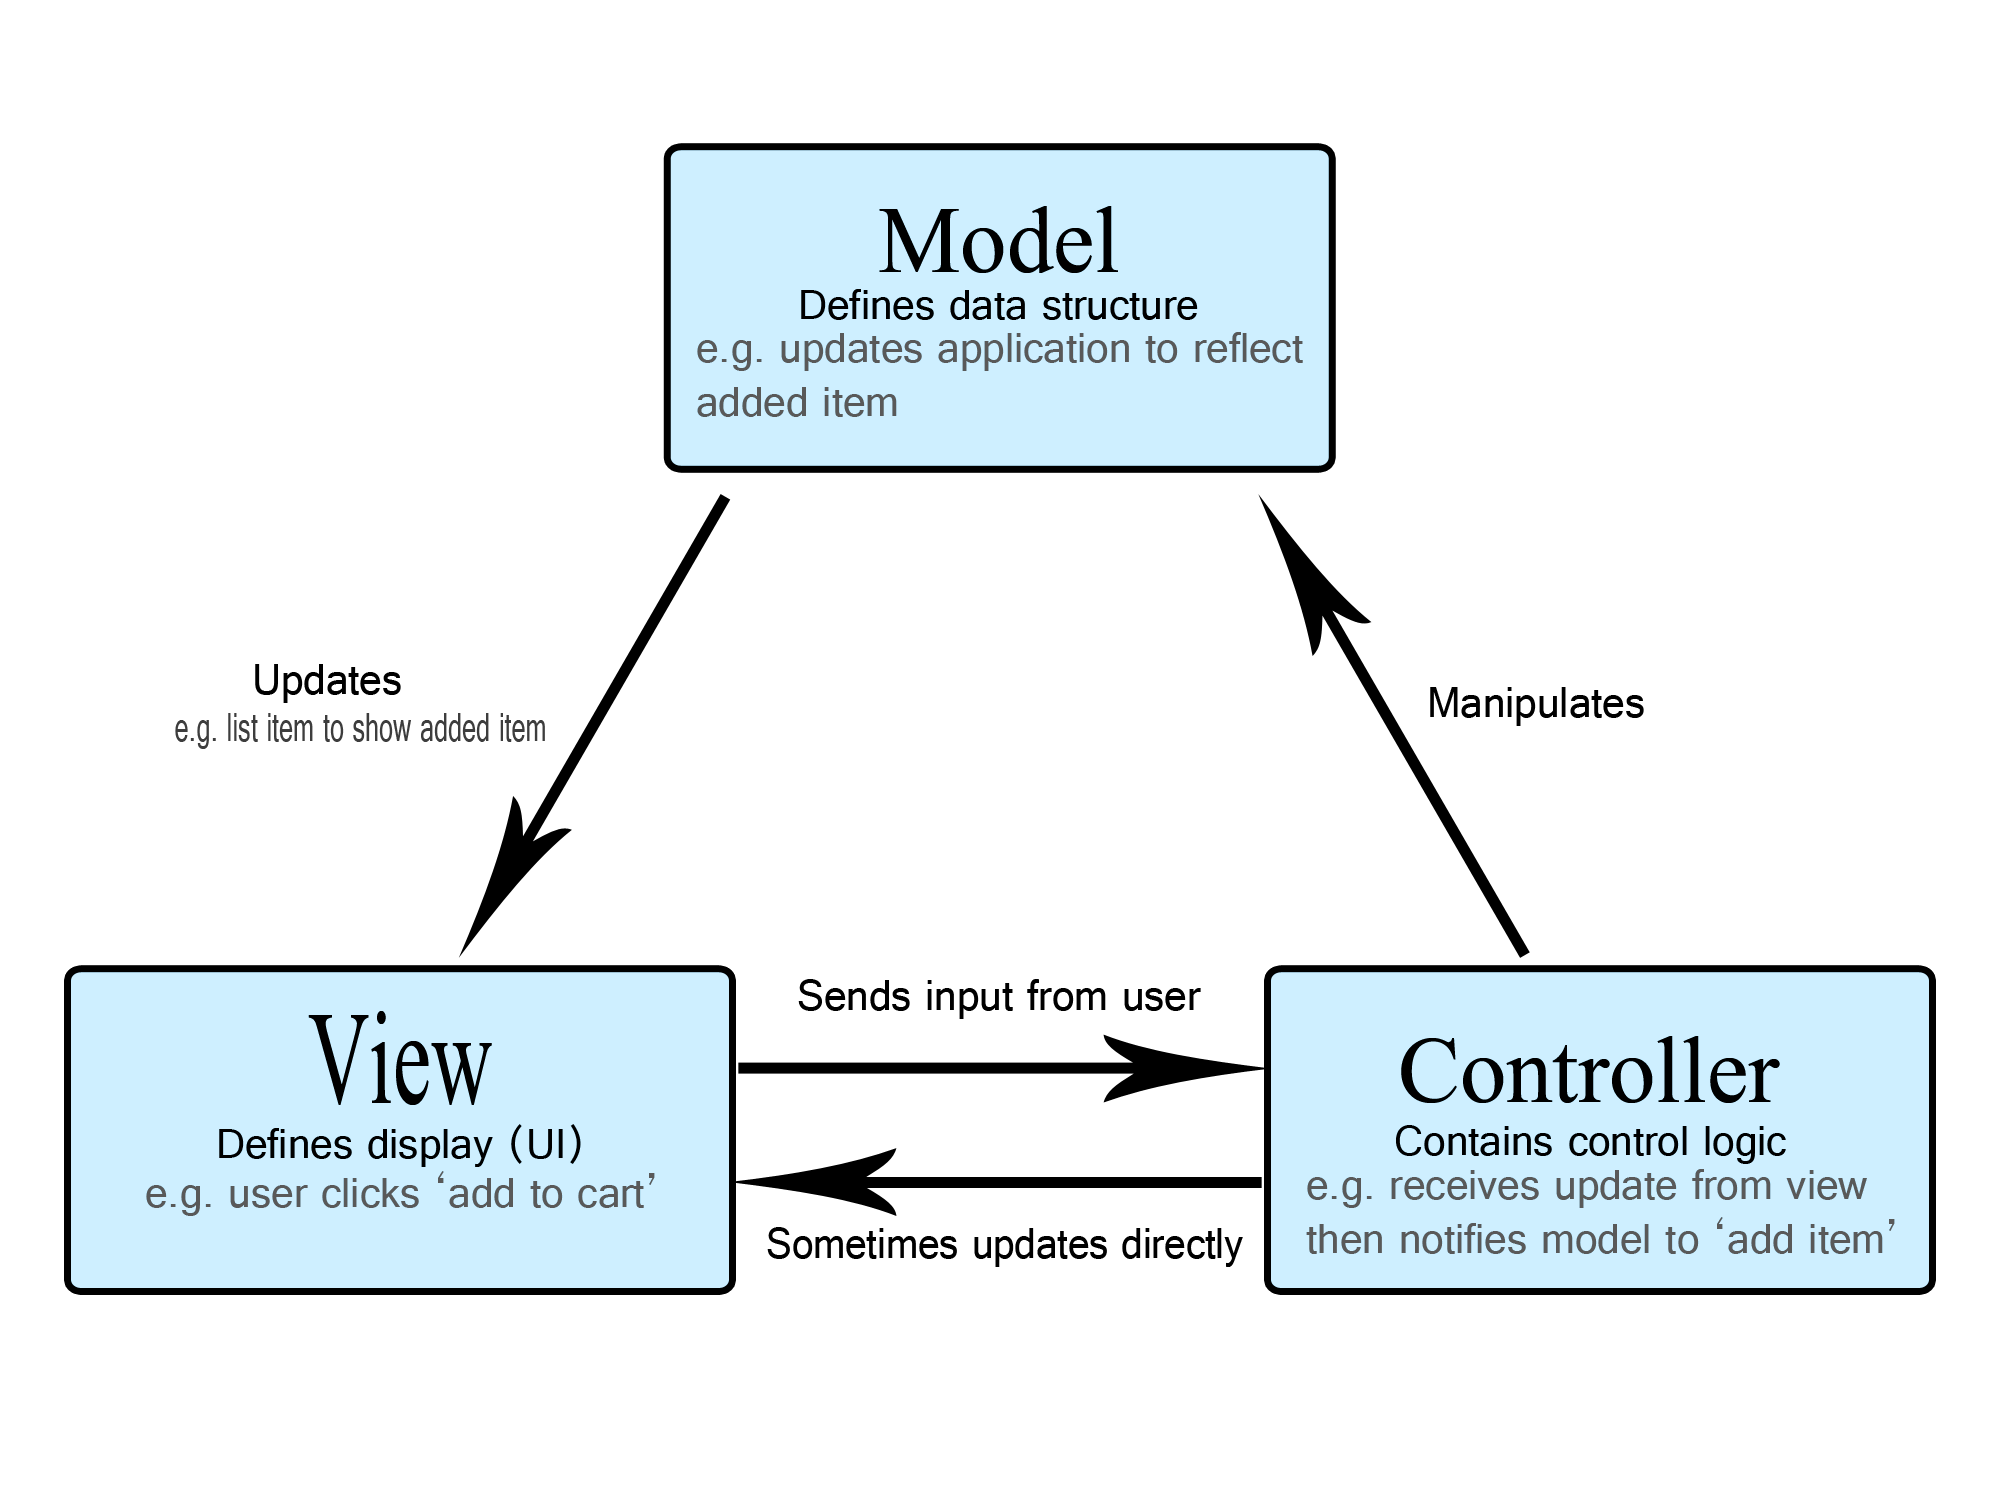
\includegraphics[width = \textwidth]{MVC.png}


\subsubsection{Detailed Architecture and Design}

\paragraph{Presentation Layer}
The presentation layer involves the components that the user sees, mainly the interface of the system. This regards the front end components which run on the client side of the system.\\ The main goal of the here is to design a visually appealing, user friendly interface design. It needs to be easy to navigate, and well constructed so as to prevent confusion when using the system.\\ There must be a good, logical ‘flow’ between screens. This would primarily work as follows: a login screen, then home course page, then marks display page for that selected course.\\\\ \textbf{1.The Login Screen}\\On this screen, access is only granted when a user enters their student number (ID login for administrator), and password associated with their account.\\Then, depending on the type of login, once the system has verified the login credentials, the user is directed to the appropriate ‘home’ page.


\includegraphics[width = \textwidth]{img.jpeg}
\textbf{2.Home Course Page}\\The content displayed on this page depends on what user logged in. It is separated into student and admin, for simplicity purposes.\\\\\textbf{Student:} When the student is directed to the course home page, they are presented with content displaying the courses they are currently enrolled in (and thus able to access, view, and query).


\includegraphics[width = \textwidth]{img.jpeg}
\textbf{Admin:}Once admin is granted access, their ‘home’ page shows a list of current courses. On this page, they can either gain access to an existing course, or add a new course, which they are then responsible for. If they choose to ‘add a new course’, the page may need to be refreshed, before the new course is shown on the ‘existing courses’ list.\\\\Once they select a specific course, they are granted many options, which will affect the course that they have selected, only.\\\\When a course is selected, the system will then display an ‘overview’ of that course.\\\\On this ‘overview page, the admin will have certain features they can access.\\\\ Their options will include:
\begin{itemize}
\item Being able to enrol, or remove a student from that specific course.
\item Editing or adding marks for an assessment that exists.
\item Add an assessment, and selecting the weighting of it (the percentage contribution to the total course mark).
\item View the current student marks for existing assessments.
\end{itemize}


\includegraphics[width = \textwidth]{img.jpeg}

\newpage
The logical flow of the system, based on the option selected by the user would look as follows:


\includegraphics[width = \textwidth]{img.jpeg}

\newpage


\includegraphics[width = \textwidth]{img.jpeg}

\newpage


\includegraphics[width = \textwidth]{img.jpeg}






\paragraph{Business Logic Layer}
\huge\textbf{ADD HERE!!!!!!!!!!}\normalsize
The business logic layer is where the core system functionality is implemented. (Runs on client/server side?) It serves as a go between for the other two layers (i.e. input is received from the presentation layer and is passed to the data layer, and the requested information is relayed back to the presentation layer).\\\\The design of the business logic layer of the system is realised so as to enhance user experience in terms of ease-of-use, efficiency and practicality.\\\\Basic functionality is carried out as follows:...
MVC is used because...\\\\This type of system design ensures that each request made from the presentation layer is carried out by the logic layer in a well-defined process using the above mentioned process (mvc approach). The correct information is always returned to successfully complete requests.\\\\The business logic layer connects to the data layer by means of (mvc model and controller etc.) which is used whenever communication with the data layer is required.


\paragraph{Data Layer}
This layer serves as the interface to external data storage/management systems and is stored server side. It provides different levels of access to files and external systems such as databases, from which data can be retrieved or written to.\\\\Security, amongst other things, must be taken into consideration when designing the data layer and determining what type of data is being stored.\\\\As per the assumptions made in the Requirements Specifications Section (see above/link to above?), the system has access to institutions databases which grant access to student and course-related data. In addition to this, the system requires its own databases to act as persistent storage for various aspects of the student marks system.\\\\Given the above, it has been decided that the data layer can be implemented in the form of a relational database. This will maintain all of the relevant attributes,as well as provide flexibility in terms of scaling, user access control, data integrity and security as well as allow for ease-of-access using Structured Query Language (SQL) querying.\\\\The data layer interacts with the business logic layer using xxx (as mentioned in the design of the business layer, above). xxx makes use of (custom SQL queries?) to retrieve any necessary data from the database. The design of the data layer allows this data to be pulled and used in an efficient manner. \huge\textbf{ADD HERE!!!!}\normalsize

\subsubsection{Class Diagram}
The class diagram is an accurate description of the code that will be produced. The class diagram aids in identifying the relationships between the different classes which we implement in the system.


\subsection{Pair 1: Front End Design}
The front end pair are responsible for the design and implementation of the presentation layer. The focus of the front end is delivering an interface that provides a good user experience while also providing an aesthetically pleasing interface. This involves creating wireframes of the relevant screens. These screens are then turned into an actual interface design. Once the design is complete, it is checked to ensure that key system logic can be implemented so as to satisfy the functional and non-functional requirements relating to it. After the front end is completed, it is then integrated with the back end, described below.

\subsection{Pair 2: Back End Design}
The back end pair are in charge of the business logic layer as well as the data layer. The use cases of the system must be translated into a class diagram. This will allow the relevant functions and procedures to be designed accordingly. Based on the class diagram the data layer can be designed by deciding what is required to be stored in the database as entities as well understanding the relationships between these entities (primary and foreign key relationships).
\section{System Implementation}

\subsection{Presentation Layer}
The presentation layer is implemented in a simplistic manner to ensure that each page is clear in function. This allows the user clarity on where he/she is and how to carry out the necessary functions (adding, viewing, changing and removing). The interface is implemented to maximise usability thus improving the user experience by allowing quick completion of tasks. While user experience is the focus, an aesthetically pleasing and minimalistic approach is used to create a good looking user interface. These components of the interface make the system seamless to use for all users. In order to achieve the above mentioned, it is required to add the necessary components (buttons, tables, graphs, scroll bars, etc) where they are required, but we must ensure we don’t ‘overwhelm’ the user, thus maintaining the minimalistic approach. As the system will be new, and users will not have experienced it before, we will take a ‘build up’ approach with regards to the presentation layer functions. By this, we mean that in the initial system, we will ensure the core components are included, to allow basic functionality to be carried out, without any confusion. As we improve on the system, rectify any flaws, and update the system, we can then begin implementing new features in the system. By doing this approach, we allow the user to be comfortable with using the system, as well as allowing them to identify what key features they believe would best benefit the system. By allowing the actual users of the system to be involved in the developmental process - by means of giving input towards system design and functionality, we allow the system to have the most relevant features, achieving a better user experience.\\ The front end developers followed the design of the mockups from the design phase and implemented them using HTML and CSS. The Bootstrap library along with Scaffolding (contained in the MVC framework) was used in depth in order to minimise the implementation.\\\\The flow between pages has been done in a logical manner to make the system quick to learn for all users as soon as deployment occurs. This will allow us to achieve the above mentioned, so as to allow users to be ‘confident’ when navigating and using the system. The interface implementation is further explained in sections below, divided into the different interface pages.

\subsubsection{Login Page}
The login page comprises of a simple form requiring an id, password and type of user (being either Student, Course Coordinator, or School Administrator). Once correct credentials are entered, the student will be directed to his/her course home page.

\subsubsection{Courses (Student)}
The course page for students will be their ‘home’ page. On this form, they will be able to see an overview of all courses they are enrolled in, and will be provided the option to select an individual course. This will be achieved by having a link on each course allowing them to be selected. which will then take them to the next page, the assessment page. The user will also be able to log-out from this page.

\subsubsection{Assessments (Student)}
The assessment page will show all marks for all types of tests (tutorial tests, class semester tests, exams, lab exams, etc) that are associated to this user, for the course which they selected on the previous page. There will not be the option to select a test, as this serves no purpose. From this page, the only options provided to the user are to return to the course home page, or to select a specific assessment mark and be able to query it. This is made possible by having a ‘Query’ button associated to each assessment, where the user will simply click on the button to submit  query to the course coordinator.\\\\The user will also be able to log-out from this page.

\subsubsection{Courses (Course Coordinator/School Administrator)}
The course coordinator and school administrator will both be redirected to the same ‘home’ screen, upon successful login. This has been done both for simplicity, and due to the fact they have a very similar set of administrative privileges, as defined in the use case diagram.\\\\The easiest way to separate and restrict access to certain functions, specifically with regard to the student offenses, is to simply disable the functionality of the respective buttons, for that user.\\\\On their home page, there will be buttons and/or drop down bars to allow the user to:
\begin{itemize}
\item Select an existing course
\item Add a new course
\item Access Plagiarism offenses
\end{itemize}
If they create a new course, they will need to enter the course details, including: course name, description, etc. Once this is done, the user may need to refresh the page in order for the new course to be added to the list of existing courses.\\\\For the School Administrator, they will have the above option, but this is not their primary role or function, and so the 2 primary functions that are available to them will be:
\begin{enumerate}
\item To select a course and be able to view statistics on it. I.e Be able to view average course marks, student comparative marks for a particular assessment, and other useful statistical results which we deem are necessary to present to the user. (This data and results shown can be improved/changed on the next iteration of the system, if it is deemed necessary by the School administrator).
\item View offenses against students. The most user-friendly way to do this, is to have a list of all students who have a/an offense(s) against their name, and then be able to view that particular student and see the nature, and number of offense(s) against them.
\end{enumerate}

\subsubsection{Assessments (Course Coordinator/School Administrator)}
The user will be guided to this page after selecting a specific course from the above mentioned courses page.\\\\When the user selects an existing course, they will then be directed to a page which shows the overview of that course, including: course description, number of students enrolled. There will be a number of options on this page, namely:
\begin{itemize}
\item Add/remove students to/from the course.
\item Create a new assessment. 
\item Upload marks for a specific assessment.
\item Edit existing assessment marks.
\item View Course report.
\item View student mark queries (specific to School administrator).
\end{itemize}
The user can then select one of the above options to implement an update to the selected, existing course data.\\\\The user is also able to logout from this page.
\subsubsection{Reports (Course Coordinator/School Administrator)}
The user is directed to this page when selecting the view course report option on the assessment page (described above).\\This page shows ‘read-only’ information, as it is a direct output of the data (marks) currently stored in the database, and applying to that specific course.\\The type of statistical information that will be shown here includes:
\begin{itemize}
\item Number of students enrolled in the course.
\item Number (percentage) of students passing the course - obtaining over 50\%
\item Individual assessment information (including average mark for the assessment, \% of students that failed, \% of students who achieved distinctions).
\end{itemize}
In order to give a good, summarised overview of a particular course or assessment, graphing will allow an easily interpreted, overview of that. Thus, it will be available as part of the report page.

\subsubsection{Offenses \& Reports (School Administrator Specific)}
This page is accessible from the course home page, when logged in as an administrator. The purpose of this page is to be able to view ‘problematic’ students. The page will provide an overview of all students who have plagiarism offenses recorded against them. This is a most useful approach rather than selecting students with offenses from within a specific course, as the focus here is the student and offenses, not the course.  As described in the core use case section, the 3 available queries apply to the student, not course specific.


\subsection{Business Logic Layer (BLL)}
The business logic layer functions as the ‘middle-man’, connecting and allowing data to flow between the presentation layer  and the data layer. From the presentation layer, when a user selects a specific course, that information is sent via the BLL, to the data layer, requesting the data pertaining to that course to then be sent back to the presentation layer, where it is manipulated and used to display useful information. Similar requests and processes exist for all the functions that need to be executed in the presentation layer. \\\\The BLL concerns the automating of processes which need to execute, between the presentation and data layer.


\subsection{Data Layer}
\huge\textbf{ADD HERE!!!!!!!!!!!!!!!!!}\normalsize
In its most simplistic form, the data layer concerns how the database is connected to the business logic layer. For our system, we created a database using XXX. It was then implemented using XXX which provides the capability for it to connect to the above mentioned layer.     

\subsection{Dependencies}
\huge\textbf{ADD HERE!!!!!!!!!}\normalsize
For the purpose of efficiency and accuracy, wherever possible, we will make use of already existing libraries in order to design, create, and implement our system.


\subsection{Testing}
\huge\textbf{ADD HERE!!!!!!!!}\normalsize
In  order to ensure our system worked and functioned correctly, we implemented a variety of test case situations. Most of these test cases were developed and tried once the system was ‘completed’. The reason it was done this way, was that we identified improvements to implement from our design phase to the implementation phase, and so in order to make sure we had successfully achieved this, we used the test cases.\\\\The test cases allowed us to see that the correct output was displayed to the user for a number of given inputs.\\\\The below describes some of the test cases we made use of to ensure the system had optimal functionality:\\\\Student:
\begin{itemize}
\item When selecting a course from the ‘home page’, the user is redirected to a page displaying all marks for that specific course. 
\item When viewing a specific mark, the user is able to click ‘query’, and this sends a notification to the course admin indicating a potential error on this specific mark.
\end{itemize}
Admin (Course \& School):
\begin{itemize}
\item On completion of adding students to a course, once refreshed, that course shows the updated student enrollment list.
\item \huge\textbf{ADDHERE!!!!!!!!!!}\normalsize
\end{itemize}
General:
\begin{itemize}
\item When logging in, and selecting type of user, we ensured that access was only granted when there was a triple-authentication match. This meant that username and password matched, and then that these login credentials matched the user-type that was indicated on the login page (student/course-coordinator/school-administrator).   
\end{itemize}



   

% % % % % % % % % %
% % % % % % % % % %
\section{SCRUM Milestones}

\subsection{Project Sprint Planning}

\subsubsection{Team}
The team was split up into the following: Project owner, SCRUM master, and the developmental team, which was further divided into front and back-end roles.\\\\Project Owner: As this task forms part of an overall course assessment, the lecturer - Professor Ekow Otoo, is assumed to be the project owner. Instruction and guidance as to the correct design, implementation, and report of the project was given, and additional support was provided by means of the project brief, consultations and emails.\\\\Scrum Master: This contributor was simultaneously our Team Lead. The role was fulfilled by Zakiya Safi. This role included ensuring sprints were completed on time.\\\\Development Team: The project was taken on by four members in total. Thus, the team was equally divided into 2 front-end developers, namely: x and y. The back-end was developed by i and j.\huge\textbf{ADDHERE!!!!}\normalsize



\subsubsection{Sprints}
It was decided to break the project down into 4 distinct sprint runs. The aim was to allocate an equal time to each sprint run but this could vary according to product complexity, risk assessment, and degree of oversight desired within each sprint run.
Following the completion date of each sprint, a short period of time is allocated to a ‘sprint break’. During this time, a review of the completed sprint will take place. This involves examining the success of the sprint run, and improving any areas of concern, before moving on to the next sprint run.\\\\\textbf{Sprint 1:} Scheduled to begin on August 6th, and be completed by the 20th of August.
\textbf{Sprint 1 rest:} 21st of August - 22nd of August.\\\\\textbf{Sprint 2:} Scheduled to begin on August the 23rd, and be completed by the 6th of September.\\
\textbf{Sprint 2 rest:} 7th of September - 8th of September.\\\\\textbf{Sprint 3:} Scheduled to begin on September 9th, and be completed by the 23rd of September.\\
\textbf{Sprint 3 rest:} 24th of September - 25th of September.\\\\\textbf{Sprint 4:} Scheduled to begin on September 26th, and be completed by the 4th of October.\\
\textbf{Sprint 4 rest:} 5th of October - 6th of October.


\subsubsection{Stand Ups}
Stand up meetings were held for 15 minutes on the first day of every sprint and every Wednesday. Due to timetable constraints and subject to availability, meetings on other days were done through messages and emails to keep everyone updated on the project.


\subsubsection{Detailed Sprint Execution}

\paragraph{Sprint 1}
This was our initial sprint. During it, we focused on tasks that would allow the best setup of the project. The aim here was to ensure that we considered all requirement aspects of the project, allowing us to prioritise the order in which we created the system, and went about the development. \\\\This included:
\begin{itemize}
\item The initial design definition: This process allowed us to identify who was going to be responsible for what parts of the system development (workload allocation), according to our areas of expertise and knowledge.
\item We identified the group lead.
\item We set in place when we would have meetings (in order to ensure we kept on track, and that all members were up-to-date with the system development progress).
\item Defining our input and output requirements of the project (based on our SRS document).
\item Identified what the key features we needed to incorporate into the system were.
\item Formulated the project name.
\item Setup our resource network, including our GitHub repository, and creating a Google Drive folder, enabling us to collaborate easily, and efficiently.
\end{itemize}

\paragraph{Sprint 2}
The second sprint mainly concerned requirement aspects of the system. This involved further developing our ideas defined in Sprint 1, and then to formally define developmental aspects of the project.\\\\The process involved:
\begin{itemize}
\item Developing the software requirement definition.
\item Formalising our project description. This allowed us to have a detailed plan of what our system needed to do, so that we had a ‘model’ on which we would define and create our system.
\item Define the project assumptions. Doing this enabled us to know what requirements we needed to consider, which would be assumed (i.e. users roles and ability to use the system), and what features we would omit (based on requirements). We incorporated prior knowledge, as well as research to make informed decisions.
\item Defining the Project Scope.
\item Formulating Use Cases. This allowed us to identify how the users (actors) would interact with the system.
\item Defining the Database: This included designing the database, identifying necessary tables, developing keys, describing rules for database implementation (NULLS, removing entries, etc.).
\end{itemize}

\paragraph{Sprint 3}
The penultimate sprint focused on the split between front-end and back-end tasks. This sprint thus required the team to be split into the front and back-end roles that were defined in Sprint 1, and to work according to this.\\\\In this sprint, we took what had been previously defined and introduced in the last Sprint, and further developed these system components. This meant we took the theoretical development, and created practical results from it during this sprint.\\\\Front-end:
\begin{itemize}
\item Interface design: by this point we had already defined how the system should work and flow, and so we not created the actual interface based on this.
\end{itemize}
Back-end:
\begin{itemize}
\item Database: We had, by this point, identified the relational entities that needed to be defined, as well as how the various tables and structures needed to interact with each other. We therefore created the actual database system at this point, adhering to the design we had earlier constructed.
\end{itemize}

\paragraph{Sprint 4}
The final sprint involved integrating the now existing front and back-ends of the system, as well as finalising and completing the report documentation.\\\\\textbf{System:} As mentioned, at this point, we had completed the initial front-end and back-end system components, and so we combined them to achieve the first instance of our working system. This required incorporating the requirements we had previously specified and making sure that the system adhered to this, as well as the features we were required to include, were in the system, and worked.\\\\\textbf{Reporting:} Throughout the design and development of the system, we were basing the system on our documentation. However, as requirements, time deadlines, and ability dictated, we updated and altered the report to incorporate the system which was actually developed. We kept track of changes during the process, and included these in the final documentation.

\subsection{Project Sprint Retrospective}
\begin{tabular}{|p{1cm}|p{1.2cm}|p{1.2cm}|p{3.7cm}|p{3.7cm}|p{3.7cm}|}
\hline \textbf{Sprint} \# & \textbf{Start} & \textbf{End} & \textbf{Success Areas} & \textbf{Concern Areas} & \textbf{Improvements}\\
\hline Sprint 1& 6 Aug & 20 Aug & Project definition done properly, roles allocated, team in agreement about approach. Repository setup and methods in place to collaborate effectively. & Team worried about being able to achieve full working system in time constraint. & Adhere to the process that is defined. When concerned, approach group and resolve issues to maintain efficiency. This maintained cohesion. \\

\hline Sprint 2 & 23 Aug & 6 Sept & Expanding on project requirements done comprehensively. Project report updated to reflect current position in project. & Due to other commitments, sprint meetings could not be carried out, in person, every Wednesday as defined. & Allow the approach to be flexible to incorporate changes. This included using ‘online meetings’ as legitimate, informative meetings.\\
\hline Sprint 3 & 9 Sept & 23 Sept & Front-end interface was designed as per specification.
Back-end database was correctly defined. Communication worked well, despite not always meeting in person. & Concerns over whether the system would be integrated correctly, specifically concerning combining front and back-end systems. & Instead of conforming to front/back end split, if possible to help on an end requiring more work, do so. \\
\hline Sprint 4 & 26 Sept & 4 Oct & System integration worked, project report was comprehensive and completed. & System is not ready to be ‘published’. A few features still to be added before releasing. & Define a simpler model in SRS in order to achieve successful development. Rather add features as time permits. \\
\hline
\end{tabular}

% % % % % % % %
% % % % % % %

\section{Conclusion}
The details regarding the design and implementation of a web application for a student marks system are documented above. The functional and non-functional requirements of the system have been determined and a design has then been formed. This design is expanded upon using UML models and is separated into three layers. It is implemented as a web application which, when tested, meets the necessary specification requirements. Lastly, a description is given of how the Agile SCRUM process has been followed by means of sprint planning and a sprint retrospective.

% % % % % % % % % %
\section*{Appendices}
\appendix
\section{Pair Responsibilites}

\subsection{Pair 1: Front End}
The front end developers served the primary role of developing the visual aspects of the system. This involved all features and tasks in the presentation layer, and included coding, design and documenting their workings. An important role here was to create a visually appealing, yet simple to use and navigate system, to give the best user experience.    
\subsection{Pair 2: Back End}
Our back-end development team had the task of developing the business logic layer, and ensuring that it fetched the correct data from the data layer, when requested. This included correctly designing the database system to prevent errors when data is requested. Tasks included designing, coding and reporting all development in this aspect.
\subsection{General}
Although tasks were allocated, and roles defined from the start, when it was required, we were able to be flexible and help each other wherever necessary. This meant that we were not limited to only front end/ back end roles. A positive from making use of this approach was that all members had a very good understanding of the overall system, and so when troubleshooting, we were able to more easily identify and rectify errors.



\end{document}